\documentclass[10pt,a4paper,twoside,twocolumn,openany]{book}
% we'll need the old hline later
\let\oldhline\hline

\usepackage[bg-a4]{dnd} % Options: bg-a4, bg-letter, bg-full, bg-print, bg-none.
\usepackage{ifxetex}

\ifxetex
	\usepackage{fontspec}
\else
	\usepackage[francais]{babel}
	\usepackage[utf8]{inputenc}
\fi
\usepackage[most]{tcolorbox}
\usepackage{caption}

\begin{document}

\begin{tikzpicture}[remember picture,overlay]
\node[inner sep=0pt] (background) at (current page.center) {
\includegraphics[width=\paperwidth,height=\paperheight]{twilek_red.jpg}};
\draw (current page.center) node [fill=yellow!30!white,fill opacity=0.6,text opacity=1,inner sep=1cm]{\Huge\centering\bfseries\sffamily\parbox[c][][t]{\paperwidth}{\centering Sib\\[15pt] % Book title
{\Large Celui qui sait obéir saura ensuite commander.}}};
\end{tikzpicture}

\chapter{Sib Morh Koh Mustafar}

\section{L'enfant de Mustafar}

Née sur la planète rouge, Sib y a vécu toute sa jeunesse. Issue d'une famille
bourgeoise, son père est un ancien militaire décoré sensible à la force, reconverti en negociant.

Mais très tôt Sib est repérée comme une utilisatrice de la force, bien plus douée que son père. Elle intègre
un établissement spécialisé dans la formation de jedi. Ce n'est pas à proprement parlé une académie car elle n'est pas officiellement approuvée par le conseil jedi mais la bordure exterieure jouit d'une certaine autonomie et donc d'une certaine liberté.

\begin{commentbox}{}
Son nom: litéralement Sib Morh de Mustafar. Les habitants de cette planète sont souvent très fiers de prosperer dans un
environnement aussi hostile et il n'est pas rare qu'il mentionne leur plannète dans leur prore nom de famille.
\end{commentbox}

\section{Un potentiel mal exploité}

Sib est une adolescente rebelle, irrespectueuse et souvent feignante. Persuadée qu'elle possède un don hors du commun elle néglige sa formation et s'attache surtout à s'amuser et se divertir.

Elle entre réguièrement en conflit avec ses formateurs, mais les connections et l'influence locale de sa famille font qu'elle est rarement inquiétée. Jusqu'au jour ou agacé son père décide de la retirer de l'établissement et de la faire travailler pour l'entreprise familiale.

Mais une fois de plus Sib n'en fait qu'a sa tête et se revèle être une pière négociante.

\section{Au service de Doku}

Alors qu'elle faisait semblant de travailler, le transport de matière première qu'elle "accompagnait" (elle avait un faible pour l'un des conducteurs) se fait attaquer. Les braconneurs ne s'attendaient probablement pas a faire face a un apprenti jedi, et Sib se montra sans concession, tuant deux des assaillants et faisant fuir le reste de la bande à elle seule.   

Un droide de sécurité appartenant au destinataire du convoi fut témoin de la scène. Il en référa à son propriétaire, un certain Maître Doku. Celui-ci contacta la famille de Sid et proposa à son père de terminer sa formation.
Etrangement Sib accepta sans hesiter, quelque chose la fascinait chez Doku, elle lui trouvait un charisme hors du commun malgré le fait qu'elle ne le connaissait que depuis quelques heures.

\section{La séparation}
Rapidement Doku s'apperçut du potentiel relativement commun de Sib. Cendant il décida de la conserver car elle était extremement dévouée, et utile. Elle acceptait sans rechigner des tâches que certains apprentis Jedi auraient pu discuter...

Cependant l'admiration totalement a sens unique de Sib envers Doku laissa
place à de l'amertume. En effet elle se rendi compte avec le temps que Doku
 ne la considérait pas réellement comme son apprenti.
Sa dévotion laissa place à de la rancune. Soucieux d'eviter un conflit imminent, Doku se debarassa de Sib en
l'assignant à un groupe de mercenaire venu sur Eriadu proteger une negociation importante.

\begin{commentbox}{Sib en quelques points}

\begin{itemize}
\item jolie et athlétique
\item charactérielle, indépendante
\item parfois méprisante envers les faibles
\item généreuse, dédiée et motivée, pour peu qu'elle apprécie quelqu'un
\end{itemize}

\end{commentbox}

\vspace{2cm}

\begin{figure}
\centering
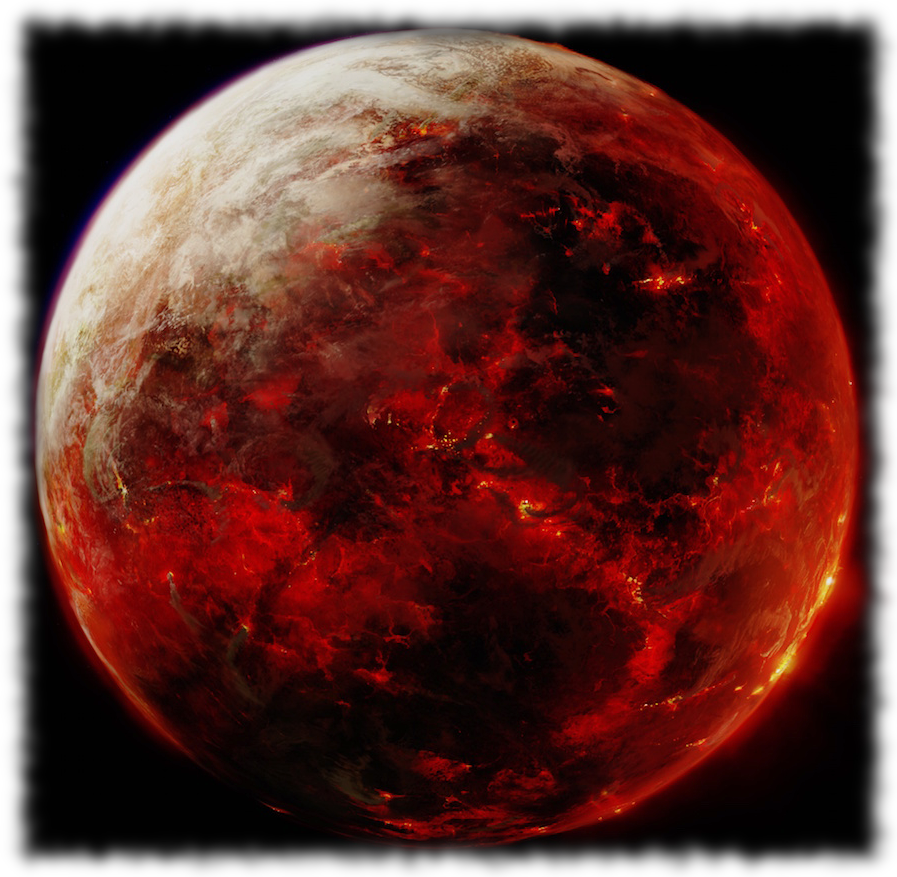
\includegraphics[scale=0.4]{mustafar.png}
\caption*{Mustafar, la planète rouge}
\end{figure}

\chapter{Chroniques}

\backgroundsetup{
scale=1,
angle=0,
opacity=1,
contents={
		\ifodd\value{page}
			\includegraphics[width=\paperwidth]{\oddbackgroundimg}
			\else
			\includegraphics[width=\paperwidth]{\evenbackgroundimg}
		\fi
		}
}

\section{Echec des négotiations}

Apres l'attentat des négotiations pour la taxation des routes commerciales, Dooku m'a conseillée de me mettre au service de Damask, qui part pour la planète Bentha. Je questionne Dooku et l'implore de me garder avec lui. Mais le divorce est consommé, il ne veut plus de moi, et moi je me rends compte qu'il ne me considère plus.

Alors j'accepte la proposition. En cadeau d'adieu il me donne un holocron. un artefact religieux censé m'apporter des connaissances.

\begin{quotebox}
L'holocron est un artefact Sith contenant une foultitude d'informations, histoire, code, 
carte galactique.
\end{quotebox}

\section{En route pour Bentha} 

J'ai finalement reussi a ouvrir l'artefact. C'est un holocron Sith contenant
une grande quantité d'informations liée aux Sith, probablement écrites par les Sith.
Les enseignements sont tres différents de ceux des Jedi.
Je suis troublée, car il semble que la vérité se trouve ni chez les Sith, et malheureseument, ni chez les Jedi.

Arrivés sur la planète, hostile, Damask nous stationons au camp pendant que Damask
et Palpatine partent en "expedition", nous n'en sauront pas plus pour le moment.
Pendant notre séjour, d'enormes eclairs de force rugissent la nuit. Le malaise de chacun est palpable.

\section{L'exploration de la mine}

Las de ne rien faire, nous décidons d'aller explorer cette mine, on suspecte
d'y trouver Damask et Palpatine. Sur le chamin nous rentrons trois bêtes féroces,
des nexus, j'ai eu beaucoup de mal a me defendre contre leurs attaques a répétitions,
mais je ne m'attendais a ce que Chavez et Dash face un carton sur les bestiaux.

Malgré l'incident nous arrivons à destination. Le coté obscure y est très puissant. 
Chavez et Dash sont pris de frissons et d'angoisse. Nous avancons jusqu'a tomber
sur une grande pièce vide. Le coté obscure y est très oppressant. En récitant
le code Sith, je decèle un cristal rouge, caché sous une pierre du mur.

\begin{quotebox}
Sib récupère un cristal rouge Sith avec lequel elle pourra construire un sabre
laser.
\end{quotebox}

Cependant nous n'arrivons pas a déplacer ou ouvrir un pan du mur.
Les traces de Damask et Palpatine sont pourtant là et prouvent que eux sont passés. 
Nous somme sur le point d'abandonner et faire demi tour quand finalement le mur se dérobe
et sortent Damask et Palpatine. Ce dernier a le visage ensanglanté mais très étrangement
ne semblke ni choqué ni dérange, il a même l'air plutôt heureux et satisfait.
Quant a Damask, il porte un large objet dans ces bras recouvert par un drap. Il fera tout
un mystère de cet objet mais je suis sure que c'est un artefact Sith. Décidément mes premières
impressions sont les bonnes, Damask et Palpatine ne m'ont pas l'air tout à fait clairs.

Affair à suivre...

\begin{paperbox}{Un choix difficile}
Sib doit faire face à un choix cornélien, quitter l'ordre Jedi et suivre sont propre
chemin ou rester loyale aux Jedi et prévenir le conseil des manigances de Palpatine et
Damask.  
\end{paperbox}


\end{document}
